\documentclass{article}

\usepackage[utf8]{inputenc}
\usepackage[greek, british]{babel}
\usepackage{alphabeta}
\usepackage{libertine}
\usepackage{csquotes}
\usepackage[backend=biber, sorting=none]{biblatex}
\usepackage{hyperref}
\usepackage{graphicx}
\usepackage{float}
\graphicspath{ {./images/} }

\pagenumbering{arabic}

\addbibresource{refs.bib}

\newcommand{\code}{\texttt}

\title{Εργασία Μηχανικής Μάθησης 2022-2023}
\author{Τσίρμπας Δημήτρης p3190205}

\begin{document}
	
\maketitle

\begin{center}
	\textit{Όλα τα ερωτήματα της εργασίας έχουν υλοποιηθεί.}
\end{center}

\section{Δομή Εργασίας}
Η εργασία χωρίζεται σε 10 αρχεία πηγαίου κώδικα python:
\begin{itemize}
	\item \code{load\_mnist.py} το οποίο εκτελεί την φόρτωση και προ-επεξεργασία των δεδομένων 
	\item \code{logistic\_regression.py} περιέχει το μοντέλο λογιστικής παλινδρόμησης
	\item \code{run\_logistic.py} περιέχει τις εντολές για την δημιουργία των γραφημάτων και αποτελεσμάτων του μέρους Β
	\item \code{mlp.py} περιέχει το μοντέλο απλού νευρωνικού δικτύου 
	\item \code{run\_mlp.py} περιέχει τις εντολές για την δημιουργία των γραφημάτων και αποτελεσμάτων του μέρους Γ (εκτός από το ερώτημα I)
	\item \code{gradcheck.py} το οποίο ελέγχει την μέθοδο backpropagation του ερωτήματος Ζ
	\item \code{sgd.py} περιέχει το μοντέλο του στοχαστικού νευρωνικού δικτύου 
	\item \code{run\_sgd.py}  περιέχει τις εντολές για την δημιουργία των γραφημάτων και αποτελεσμάτων του ερωτήματος I
\end{itemize}

Περιέχονται επίσης τα αρχεία \code{common.py}, που περιέχει κοινές συναρτήσεις για τα παραπάνω αρχέια, και \code{test\_load\_mnist.py} το οποίο συμβάλλει στην επικύρωση των δεδομένων μας.

Η πλήρη τεκμηρίωση του κώδικα και της υλοποίησης μπορεί να βρεθεί στα παραπάνω αρχεία με την μορφή pydoc και σχολίων.


\section{Μέρος Β - Λογιστική Παλινδρόμηση}

\subsection{Ερώτημα Δ}
Ο ταξινομητής μας έχει υλοποιηθεί στο αρχείο \code{logistic\_regression.py}. Η πλήρης τεκμηρίωση του μοντέλου, των μεθόδων του και των υπερπαραμέτρων βρίσκεται εκεί με τη μορφή docstrings. Η κανονικοποίηση $L_{2}$ έχει ήδη υλοποιηθεί σε αυτό το αρχείο, αλλά για τους σκοπούς αυτής της ερώτησης θα θέσουμε την υπερπαράμετρο \code{$\lambda$} ως 0, παρακάμπτοντας την.\par

Ο κώδικας για την εκτέλεση του μοντέλου βρίσκεται στο αρχείο \code{run\_logistic.py}. Θα τρέξουμε το μοντέλο με υπερπαραμέτρους \code{iter = 500} και \code{alpha = 0.2}. Το αποτέλεσμα είναι η ακρίβεια εκπαίδευσης να είναι ίση με $0.982$ και η ακρίβεια ελέγχου ίση με $0.981$. Τα πλήρη αποτελέσματα της εκπαίδευσης και του ελέγχου παρουσιάζονται στην Εικόνα \ref{logistic_train_test}.

\begin{figure}
	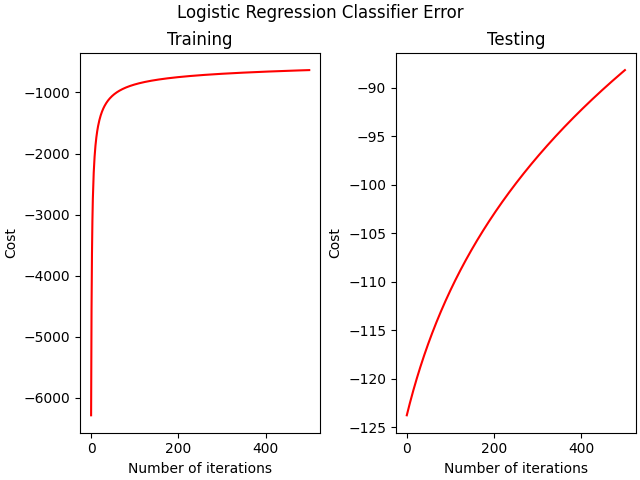
\includegraphics[width=7cm]{logistic_error.png}
	\centering
	\caption{Τα αποτελέσματα της εκπαίδευσης και του ελέγχου στον ταξινομητή μας. Αριστερά: Το κόστος εκπαίδευσης ως συνάρτηση των επαναλήψεων του αλγορίθμου gradient ascent. Δεξία: Το αντίστοιχο κόστος ελέγχου. Υπενθυμίζουμε ότι οι κλίμακες των γραφημάτων δεν είναι ίσες, καθώς ο ήδη εκπαιδευμένος ταξινομητής αρχίζει με πολύ μικρότερο κόστος. }
	\label{logistic_train_test}
\end{figure}


\subsection{Ερώτημα Ε}
Επιλέγουμε το διάστημα των \code{$\lambda$} τιμών μας λογαριθμικά, εφόσον η βέλτιστη τιμή κανονικοποίησης είναι πολύ πιο πιθανό να βρίσκεται αρκετά κοντά στο 0. Η λογαριθμική κλίμακα μας επιτρέπει να ψάξουμε πιο πολλές τιμές του \code{$\lambda$} όσο πιο κοντά φτάνουμε στο κάτω όριο αναζήτησης μας, το $10^{4}$. Η προσέγγιση αυτή χρησιμοποιείται και στην πράξη για κανονικοποίηση $L^{2}$ \cite{jerome}\par

Σημειώνουμε ότι λόγω υπολογιστικών απαιτήσεων, ο αριθμός επαναλήψεων των μοντέλων μας μειώνεται στις 250 επαναλήψεις. Κατά την εκτέλεση του προγράμματος υπάρχει επίσης πιθανότητα να εμφανιστούν ειδοποιήσεις για αριθμητική υπερχείλιση. Αυτό είναι αποτέλεσμα της επιλογής πολύ μεγάλης τιμής του \code{$\lambda$}, κυρίως στο διάστημα [8, 10]. Σε αυτό το σημείο η κανονικοποίηση είναι τόσο ισχυρή που αποτρέπει το μοντέλο μας από το να μάθει, και έτσι αυτό μαντεύει την ίδια κατηγορία για κάθε παράδειγμα ελέγχου.\par

Στην δική μας περίπτωση το μοντέλο, κρατώντας τις υπόλοιπες υπερπαραμέτρους ίσες με το προηγούμενο υποερώτημα, προτιμά την ελάχιστη τιμή κανονικοποίησης \code{$\lambda = 10^{-4}$} με  ακρίβεια ελέγχου ίση με $0.981$. Παρατηρούμε ότι η ακρίβεια ελέγχου με την επιλεγμένη τιμή \code{$\lambda$} είναι μικρότερη από την αντίστοιχη στο υποερώτημα Δ. Αυτό μας υποδεικνύει είτε ότι η βέλτιστη τιμή βρίσκεται έξω (και πιο συγκεκριμένα πριν) από το διάστημα αναζήτησης μας, είτε ότι για την διαφορά ευθύνεται το στατιστικό σφάλμα. \par

Ο κώδικας παραγωγής των παραπάνω γραφημάτων και αποτελεσμάτων βρίσκεται στο αρχείο \code{run\_logistic.py}. Τα πλήρη αποτελέσματα αναζήτησης της υπερπαραμέτρου παρουσιάζονται στην Εικόνα \ref{logistic_lambda_accuracy}.

\begin{figure}
	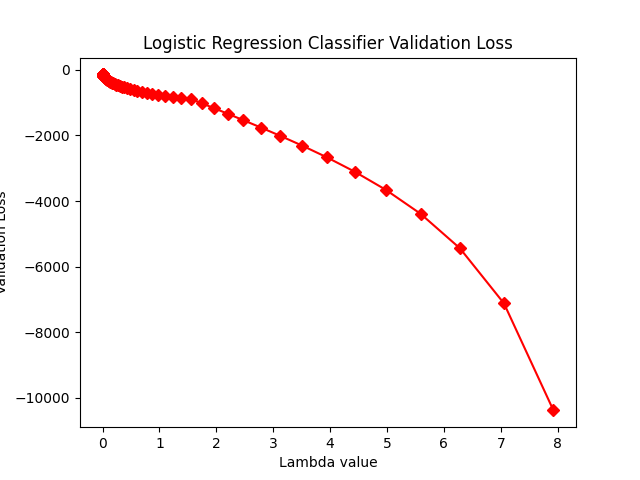
\includegraphics[width=7cm]{logistic_lambda_accuracy.png}
	\centering
	\caption{ Τα αποτελέσματα της αναζήτησης για το βέλτιστο \code{$\lambda$}. Οι ρόμβοι αντιπροσωπεύουν τις τιμές που εξετάσαμε. Παρατηρείστε το πλήθος των τιμών που εξετάστηκαν στην αρχή συγκριτικά με το τέλος του πεδίου αναζήτησής μας.}
	\label{logistic_lambda_accuracy}
\end{figure}


\section{ΜΕΡΟΣ Γ - Νευρωνικό Δίκτυο}

\subsection{Ερώτημα ΣΤ}

Το νευρωνικό μας δίκτυο έχει υλοποιηθεί στο αρχείο \code{mlp.py}. Αποτελείται από δύο πίνακες βαρών και δύο πίνακες bias:
\begin{itemize}
	\item  Ο πίνακας \code{h\_w} (hidden weights) έχει μέγεθος $IxH$
	\item  Ο πίνακας \code{o\_w} (output weights) έχει μέγεθος $HxO$
	\item  Ο πίνακας \code{h\_b} (hidden bias) έχει μέγεθος $1xH$
	\item  Ο πίνακας \code{o\_b} (output bias) έχει μέγεθος $1xO$
\end{itemize}
όπου I=\code{input\_size}, H= \code{hidden\_layer\_size}, O= \code{output\_size}. Ο κώδικας για την εκτέλεση του δικτύου βρίσκεται στο αρχείο \code{run\_mlp.py}, το οποίο εκτελεί κώδικα και για τα ερωτήματα Η, Θ.

Θα τρέξουμε το μοντέλο με υπερπαραμέτρους \code{m=2}, \code{$\eta$=0.2} και \code{tolerance=0.001}. Το \code{tolerance} είναι μια υπερ-παράμετρος απαραίτητη για το early stopping, και η οποία καθορίζει πόσο το κόστος πρέπει να έχει μειωθεί για να θεωρείται η τρέχουσα εποχή "βελτίωση". Το αποτέλεσμα είναι η ακρίβεια εκπαίδευσης να είναι ίση με $0.978$, το τελικό κόστος εκπαίδευσης ίσο με $0.0671$, η ακρίβεια ελέγχου ίση με $0.974$ και το μέσο κόστος ελέγχου ίσο με $0.0734$. Τα πλήρη αποτελέσματα της εκπαίδευσης παρουσιάζονται στην Εικόνα \ref{mlp_train_test}.

\begin{figure}
	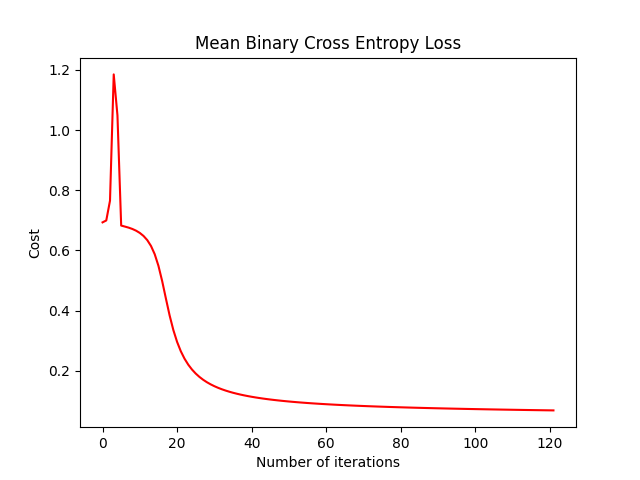
\includegraphics[width=10cm]{mlp_error.png}
	\centering
	\caption{Το κόστος εκπαίδευσης ως συνάρτηση των επαναλήψεων του αλγορίθμου gradient descent.}
	\label{mlp_train_test}
\end{figure}


\subsection{Ερώτημα Ζ}

Ο τύπος της Δυαδικής Διασταυρούμενης Εντροπίας είναι:
\begin{equation}
	\label{eq:1}
	E_{b} = -(t \ln \hat{y} + (1-t) \ln(1-\hat{y}))
\end{equation}
όπου $t$ το διάνυσμα των ετικετών δεδομένων και $\hat{y}$ το της εκτιμώμενης πιθανότητας.

Στην παραπάνω εξίσωση για να βρούμε την παραγωγό ως προς  ότι η τιμή $t$ είναι πάντοτε γνωστή, αντίθετα με τη $\hat{y}$, επομένως θα παραγωγίσουμε με βάση το $\hat{y}$. Εφόσον $y = f(x) + g(x) \iff y' = f'(x) + g'(x)$ ισχύει ότι:

\begin{equation}
	\label{eq:2}
	\frac{\partial E_b}{\partial \hat{y}} = \frac{\partial}{\partial \hat{y}} (t\ln \hat{y}) + \frac{\partial}{\partial \hat{y}} (1-t) \ln (1-\hat{y})
\end{equation}

Αναλύουμε τις επιμέρους συναρτήσεις του αθροίσματος της παραγώγου:

\begin{equation}
	\label{eq:3}
	\frac{\partial}{\partial \hat{y}} (t \ln\hat{y}) = \frac{\partial }{\hat{y}} (t\ln\hat{y}) + \ln\hat{y} \frac{\partial}{\partial \hat{y}}t = \frac{t}{\hat{y}} + \ln \hat{y} \cdot 0 = \frac{t}{\hat{y}}
\end{equation}

\begin{equation}
	\label{eq:4}
	\frac{\partial}{\partial \hat{y}} ((t-1) \ln(1-\hat{y})) = (1-t)\frac{\partial}{\partial\hat{y}} (\ln(1-\hat{y})) + \ln(1-\hat{y}) \frac{\partial}{\partial \hat{y}}(1-t) = \frac{1-t}{1-\hat{y}} + \ln(1-\hat{y}) \cdot 0 =\frac{1-t}{1-\hat{y}}
\end{equation}


Επομένως, αθροίζοντας τις \ref{eq:3}, \ref{eq:4}, η \ref{eq:2} γίνεται:
\begin{equation}
	\frac{\partial E_b}{\partial \hat{y}} = - (\frac{t}{\hat{y}} - \frac{1-t}{1-\hat{y}}) = \frac{1-t}{1 - \hat{y}} - \frac{t}{\hat{y}}
\end{equation}

\begin{figure}
	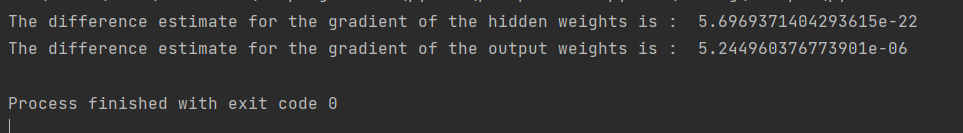
\includegraphics[width=10cm]{gradcheck.png}
	\centering
	\caption{Το αποτέλεσμα εκτέλεσης του κώδικα ελέγχου της παραγώγου στο νευρωνικό μοντέλο μας}
	\label{gradcheck}
\end{figure}

Η εικόνα \ref{gradcheck} δείχνει το αποτέλεσμα της εκτέλεσης του κώδικα ελέγχου της παραγώγου. Ο κώδικας επαλήθευσης του αναλυτικού τύπου βρίσκεται στο αρχείο \code{gradcheck.py}. Επιπλέον, εφόσον η μέθοδος που χρησιμοποιείται για τον υπολογισμό του gradient είναι \textit{ακριβώς} η ίδια και για το στοχαστικό μοντέλο μας (στον κώδικα η μέθοδος \code{\_back\_propagation}), η παραπάνω απόδειξη και αποτέλεσμα εκτέλεσης παραμένουν ίδια.


\subsection{Ερώτημα Η}

Εκτελούμε grid search για τις παραμέτρους $m, \eta$. Επιλέγουμε το διάστημα των $\eta$ τιμών μας στο χώρο αναζήτησης $[0.5, 10^{-5}]$, εκθετικά κοντά στο $0.5$ εφόσον εμπειρικά αναμένουμε ότι η βέλτιστη τιμή της θα βρίσκεται κοντά στις τιμές $0.5, 0.01, 0.01$.  το οποίο για το συγκεκριμένο δίκτυο είναι το $(\eta=0.5, m=0.5, E=172)$ με κόστος επικύρωσης ίσο με $0.0423$.

Το πρόγραμμα εκτέλεσης του grid search βρίσκεται στο αρχείο \code{run\_mlp.py}. Η αναζήτηση χρειάζεται περίπου 10 λεπτά για να βγάλει το βέλτιστο συνδυασμό υπερπαραμέτρων, το οποίο οφείλεται σχεδόν αποκλειστικά στην εκπαίδευση και επαλήθευση μοντέλων με $M \in {256, 512, 1024}$. Λόγω των περιορισμών στις υπερπαραμέτρους δεν μπορούμε να μειώσουμε σημαντικά τον χρόνο εκτέλεσης.


\subsection{Ερώτημα Θ}

Χρησιμοποιούμε την μέθοδο \code{predict} του μοντέλου μας για να αποκτήσουμε τις προβλεπόμενες ετικέτες του. Η μέθοδος αυτή χρησιμοποιεί μεθόδους της numpy, ισοδύναμες της κατηγοριοποιήσης με βρόγχο. Στο σύνολο ελέγχου το μοντέλο με τις βελτιστοποιημένες παραμέτρους επιτυγχάνει ακρίβεια ελέγχου ίση με $0.979$ και κόστος ελέγχου ίσο με $0.0569$.

\subsection{Ερώτημα Ι}

Ο κώδικας του ταξινομητή SGD μπορεί να βρεθεί στο αρχείο \code{sgd.py}.

Υλοποιούμε τον ταξινομητή στοχαστικής καθοδικής κλίσης ως υποκλάση του προηγούμενού μας ταξινομητή. Η κύρια αλλαγή είναι το πέρασμα mini-batches στην μέθοδο \code{\_back\_propagation} αντί για το σύνολο των δειγμάτων εκπαίδευσης. Πιο συγκεκριμένα, αντί να περάσουμε στην \code{\_back\_propagation} έναν πίνακα διαστάσεων 9072x784, περνάμε πίνακα Βx784 όπου Β το μέγεθος του mini-batch. Τα παραδείγματα εκπαίδευσης και οι ετικέτες τους ανακατεύονται πριν κάθε επανάληψη του αλγορίθμου έτσι ώστε το μοντέλο μας να εξετάζει κάθε φορά διαφορετικό σύνολο παραδειγμάτων. Η ίδια η μέθοδος παραμένει ίδια.


 Το πρόγραμμα εκτέλεσης του ταξινομητή καθώς και του παρακάτω grid search βρίσκεται στο αρχείο \code{run\_sgd.py}. Τρέχοντας τον ταξινομητή μας με παρόμοιες παραμέτρους με τον προηγούμενο και με αυθαίρετο μέγεθος mini-batch=128, επιτυγχάνει ακρίβεια εκπαίδευσης $0.967$ με κόστος $0.0817$ και ακρίβεια ελέγχου $0.965$ με κόστος $0.1194$. Η ακρίβεια αυτή είναι κατά μικρό βαθμό χειρότερη από τον ταξινομητή λογιστικής παλινδρόμησης, αν και λόγω του υπολογισμού με mini-batches και του κριτηρίου early-stopping, το μοντέλο είναι σημαντικά γρηγορότερο.
 
 Ένα πλήρες γράφημα για την εξέλιξη του κόστους εκπαίδευσης βρίσκεται στην Εικόνα \ref{sgd_train_test}. Παρατηρούμε ότι το κόστος του ταξινομητή μας ακολουθεί την ίδια πορεία με αυτό της Εικόνας \ref{mlp_train_test}, αν και είναι εμφανώς περισσότερο ανώμαλη. Αυτό οφείλεται στην τυχαιότητα του αλγόριθμου SGD, ο οποίος προσθέτει "θόρυβο" στη διαδικασία εκπαίδευσης μέσω του τυχαίου και περιορισμένου πλήθους δεδομένων που βλέπει το μοντέλο μας σε κάθε επανάληψη του SGD.

Δοκιμάζοντας το μοντέλο μας με τιμές $Β=2^{i}, i=1,2,..,8$, η βέλτιστη τιμή μεγέθους mini-batch φαίνεται να είναι η $B=32$, με κόστος επικύρωσης ίσο με $0.1215$ και με $Ε=52$ εποχές εκπαίδευσης. Χρησιμοποιώντας τη βέλτιστη τιμή B, μπορούμε να τρέξουμε την ίδια μέθοδο αναζήτησης βέλτιστων υπερπαραμέτρων όπως στο ερώτημα Η. Με την ίδια μεθοδολογία και το ίδιο χώρο αναζήτησης υπερ-παραμέτρων, το πρόγραμμα μας βρίσκει βέλτιστες υπερ-παραμέτρους $(\eta=0.139, m=32, E=57)$. Δυστυχώς το βέλτιστο αυτό μοντέλο φαίνεται να πάσχει είτε από overfitting είτε από κάποιο αριθμητικό σφάλμα, καθώς η ακρίβεια ελέγχου του είναι $0.618$, με κόστος $0.6304$. 

\textit{Σημειώνουμε ότι λόγω της τυχαιότητας του αλγορίθμου SGD τα αποτελέσματα της εκτέλεσης μπορεί να είναι διαφορετικά από αυτά που αναγράφονται στο έγγραφο αυτό.}

\begin{figure}
	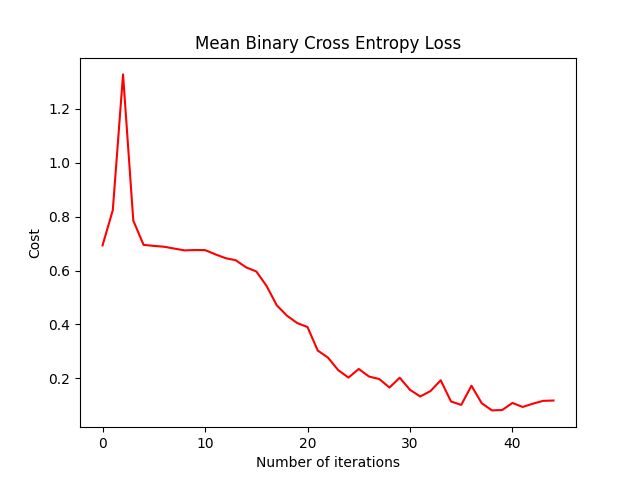
\includegraphics[width=7cm]{sgd_error.png}
	\centering
	\caption{Το κόστος εκπαίδευσης ως συνάρτηση των επαναλήψεων του αλγορίθμου stochastic gradient descent.}
	\label{sgd_train_test}
\end{figure}


\printbibliography

\end{document}